\documentclass[12pt]{article}	

\usepackage[margin=1in]{geometry}
\usepackage{amsmath,amssymb,amsthm}
\usepackage{caption}
\usepackage{subcaption}
\usepackage{graphicx}
\usepackage{url}
\usepackage{mathrsfs}
\newtheorem{theorem}{Theorem}
\newtheorem{notation}{Notation}
\newtheorem{claim}{Claim}
\newtheorem{lemma}{Lemma}
\newtheorem{definition}{Definition}
\renewcommand{\qedsymbol}{$\blacksquare$}
\newtheorem*{remark}{Remark}
\usepackage[utf8]{inputenc}

\usepackage{listings}
\usepackage{xcolor}

\definecolor{codegreen}{rgb}{0,0.6,0}
\definecolor{codegray}{rgb}{0.5,0.5,0.5}
\definecolor{codepurple}{rgb}{0.58,0,0.82}
\definecolor{backcolour}{rgb}{1,1,1}
\definecolor{grey}{rgb}{0.70, 0.70, 0.70}

\lstdefinestyle{mystyle}{
	backgroundcolor=\color{backcolour},   
	commentstyle=\color{grey},
	keywordstyle=\color{codepurple},
	numberstyle=\tiny\color{codegray},
	stringstyle=\color{codegreen},
	basicstyle=\ttfamily\footnotesize,
	breakatwhitespace=false,         
	breaklines=true,                 
	captionpos=b,                    
	keepspaces=true,                 
	numbers=left,                    
	numbersep=5pt,                  
	showspaces=false,                
	showstringspaces=false,
	showtabs=false,                  
	tabsize=2
}

\lstset{style=mystyle}


\begin{document}
	Arun Suresh
	\begin{center}
		Computational Physics 1 - Midterm Exam
	\end{center} 
	{\rule{\linewidth}{0.1mm} }

\textbf{(1 a)} The given function is $$g(x) = \bigg [\cos(5\pi x) - e^{\frac{-x^2}{2}}\sin \bigg (\frac{\pi}{2}x \bigg ) \bigg ]\frac{\sin(\pi x)}{x}$$ The function was sampled with 200 data points in between $-10$ to $10$ and is plotted below.
\begin{figure}[h]
	\centering
	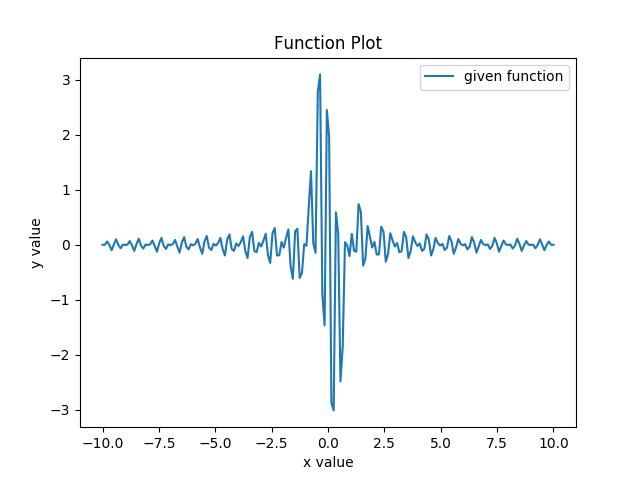
\includegraphics[width=0.75\textwidth]{functionplot200.png}
	\caption{Function Plot}
\end{figure}

\textbf{(1 b)} The derivative of the above function was calculated to be 
$$g'(x) = \bigg [\cos(5\pi x) - e^{-x^2/2}\sin\bigg (\frac{\pi}{2} x\bigg )\bigg ]\bigg (-\frac{\sin(\pi x)}{x^2} + \frac{1}{x}\pi\cos(\pi x)\bigg ) +$$ $$ \frac{\sin(\pi x)}{x}(-5\pi\sin(5\pi x) + xe^{-(x^2)/2}\sin(0.5\pi x) + 0.5\pi\cos(0.5\pi x)e^{(-(x**2)/2)})$$
This analytic solution was plotted for the same sampled data as before, and is reproduced below. 
\begin{figure}[h]
	\centering
	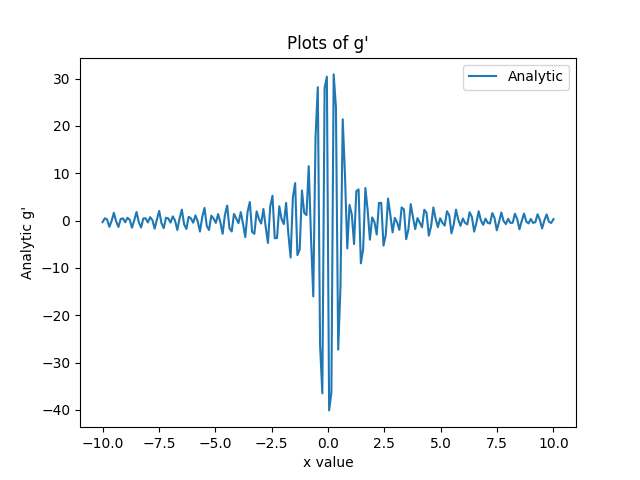
\includegraphics[width=0.60\textwidth]{gpranalytic.png}
	\caption{Analytic derivative}
\end{figure}\\\\\\

\textbf{(1 c)} The forward, backward and central difference methods were employed for the function $g(x)$ to compute the derivative. The overlapping plots of the three methods, along with the analytic solution is presented below. 
\\\\
\begin{figure}[h]
	\centering
	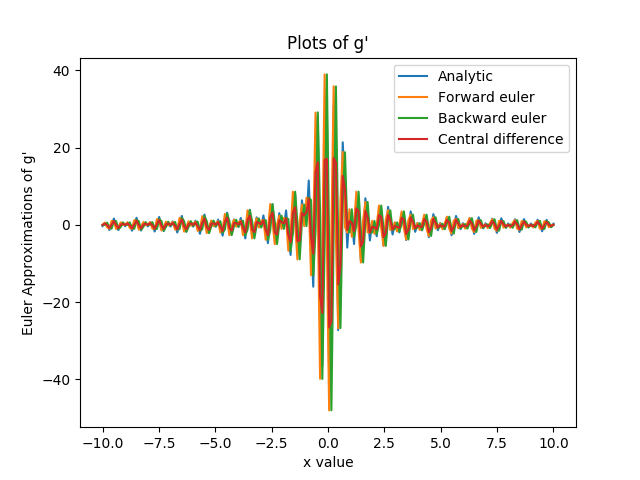
\includegraphics[width=0.60\textwidth]{gprimeeulerplot.png}
	\caption{Euler Approximations}
\end{figure}\\
The backward euler, and central difference are implicit methods because the unknown variable is on both sides of the equation, and we are essentially solving an algebraic expression to obtain our desired result. However, the forward euler uses data at current position and previous position to obtain the value at the future point - and is thus an explicit method. \\\\  
\textbf{(1 d)} Plotted below are the average and percent error with respect to $x$ 
\begin{figure}[h]
	\centering
	\begin{subfigure}[h]{0.40\textwidth}
		\centering
		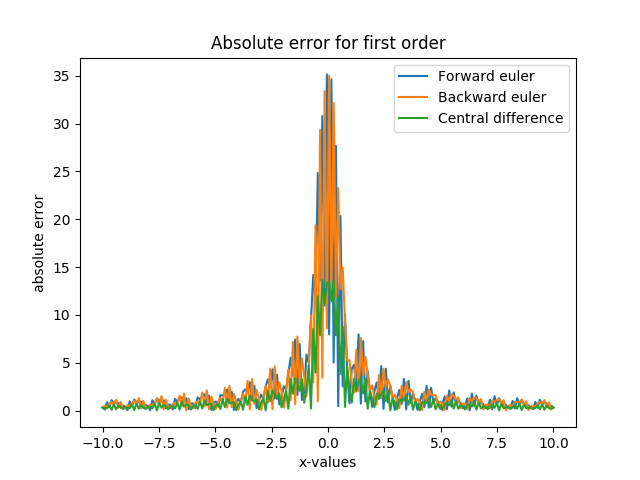
\includegraphics[width=\textwidth]{gprimeabserror.png}
		\caption{Absolute Error }
	\end{subfigure}
	\begin{subfigure}[h]{0.40\textwidth}
		\centering
		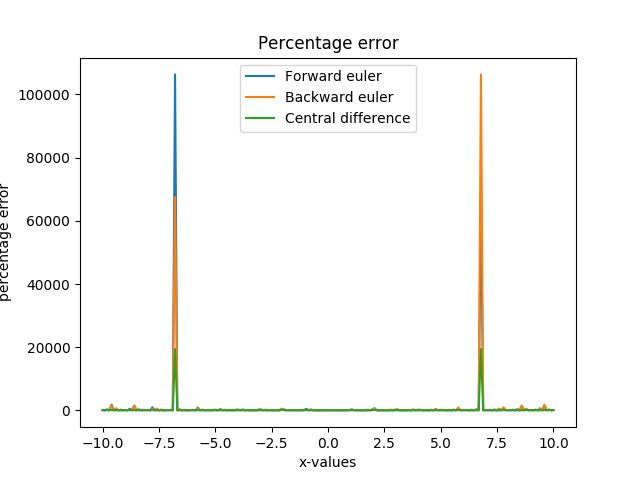
\includegraphics[width=\textwidth]{gprimepercenterror.png}
		\caption{Percent error}
	\end{subfigure}
	\caption{Error Plots}
\end{figure}\\\\
It is clear that the central difference method performs much better than both foward and backward euler methods.  This is because, the signal ($g(x)$) given rapidly changes and is very sensitive to changes in $x$. So, the forward and backward euler methods that rely on next and previous data point overestimate and underestimate the derivative value by a huge amount. The central difference, being an average of the two, performs better. Notice however, that due to the erratic behavior of the function close to zero, the averaging out process in central difference fails to capture the peaks properly; this is where most of the errors occur.\\\\
The spikes that can be noticed in the percentage error from backward and forward euler methods, seem worrysome - and should be normalized properly, however, at the risk of losing insight. The spikes exist because at those two $x$ values, the analytic derivative gets very close to zero, while the euler approximations aren't as close. The difference between the analytic value and the real value is on the order of 1.50, while the orignial analytic value there is $0.001743$, and so upon dividing the two numbers, we have results in the order of $1500$, and when multiplied by 100, we obtain the huge number that we observe. I believe these spikes are specific to the sampling of $x$ values. Given a different initial point, we could have more spikes or less depending on how many $x$ values are sampled where $g'(x)$ is very close to zero. We could also reduce the amount of error we have by increasing the resolution of the data (getting more data points)\footnote{we will observe this in part 1 f}\\
The average errors (for Forward Euler, backward Euler and central-difference respectively) reported are as follows 
\begin{figure}[h]
	\centering
	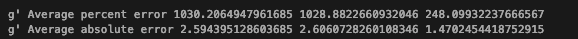
\includegraphics[width=0.60\textwidth]{error200gpr.png}
	\caption{Average errors}
\end{figure}\\
\textbf{(1 e)} \\ The same steps as above was done for computing the second derivative of the function.\footnote{for the sake of sanity, I refrain from reproducing the analytic second derivative}. Plotted below is the analytic second derivative. 
\begin{figure}[h]
	\centering
	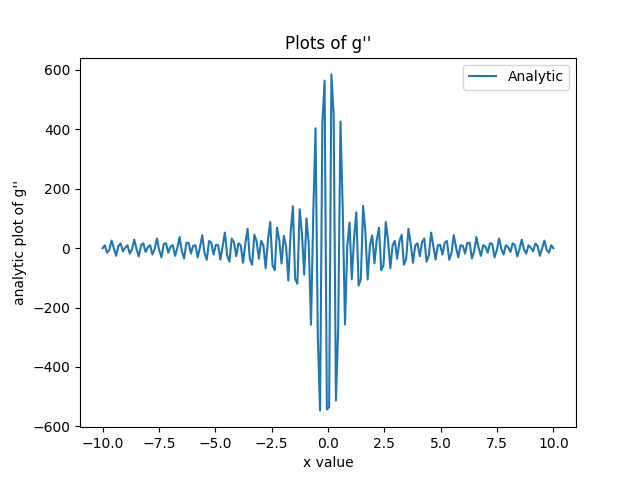
\includegraphics[width=0.55\textwidth]{gdpranalytic.png}
	\caption{Analytic plot of g''}
\end{figure}\\ This looks promising because, it looks like a flipped and scaled up version of $g(x)$, which is what we would expect out of a second derivative of a function that has $x^2$'s, sines and cosines as its main components. The forward, backward and central difference methods were employed for the function $g'(x)$ to compute the derivative. The overlapping plots of the three methods, along with the analytic solution is presented below (Figure 7). 
\begin{figure}[h]
	\centering
	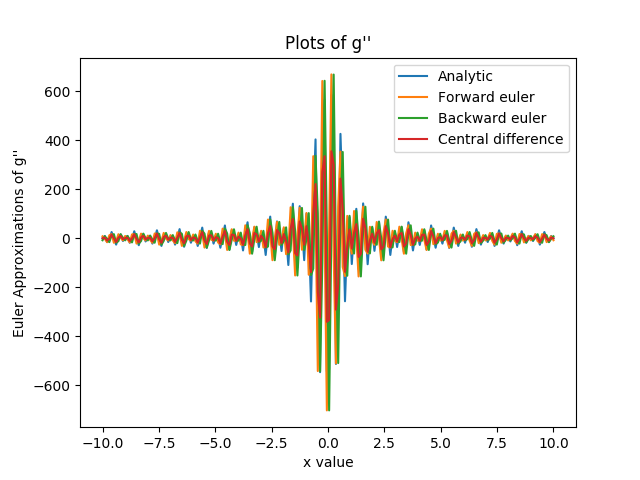
\includegraphics[width=0.60\textwidth]{gdprimeeulerplot.png}
	\caption{Euler Approximations}
\end{figure}\\\\
Plotted below are the average and percent error with respect to $x$ (Figure 8)
\begin{figure}[h]
	\centering
	\begin{subfigure}[h]{0.40\textwidth}
		\centering
		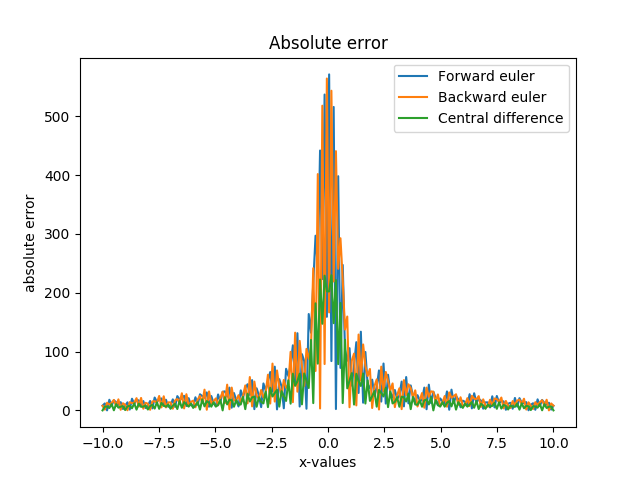
\includegraphics[width=\textwidth]{gdprimeabserror.png}
		\caption{Absolute Error }
	\end{subfigure}
	\begin{subfigure}[h]{0.40\textwidth}
		\centering
		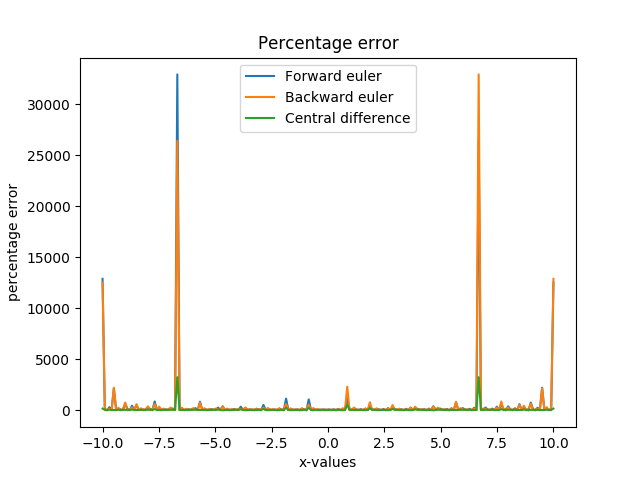
\includegraphics[width=\textwidth]{gdprimepercenterror.png}
		\caption{Percent error}
	\end{subfigure}
	\caption{Error Plots}
\end{figure}\\\\
It is clear that, once again the central difference method performs much better than both foward and backward euler methods, for the same reasons as before (in fact, $g'(x)$ is even more sensitive than $g$)\\\\
We notice more spikes in the percentage errors here, because like we noticed $g'(x)$ varies very rapidly, and thus will have a lot of points where it plummets to zero. Forward and backward euler methods do not particularly work well in this scenario, and thus resulting in huge spikes with a comparably lesser magnitude than the ones in the case of $g'$. 

The average errors (for Forward Euler, backward Euler and central-difference respectively) reported are as follows 
\begin{figure}[h]
	\centering
	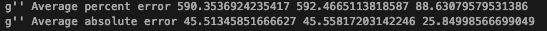
\includegraphics[width=0.60\textwidth]{error200gdpr.png}
	\caption{Average errors}
\end{figure}\\\\
We notice that the average percent error has significantly gone down from the case of $g'$, but the average absolute error has significantly gone up. This can be because of the additional scale factors that we obtain upon taking the second derivative - and so the absolute errors naturally scale up. However, the percentage errors scale down because - now we have a positive scaling to the function values (and especially to the ones close to zero), and thus division by the new analytic values do not cause huge errors to crop up - like it did in the case of $g'$. One other thing to notice is that in both cases - areas with most absolute errors do not have a relatively huge amount of percentage errors because the values close to the origin are more often away from zero, and thus no huge scaling occurs in that region, and we get a desirable percentage estimate. \\\\

\textbf{(1 f)}
The number of grid points was increased to 400, and with this, I was able to obtain an increased degree of smoothing in the function. The function $g(x)$ is plotted below. 
\begin{figure}[h]
	\centering
	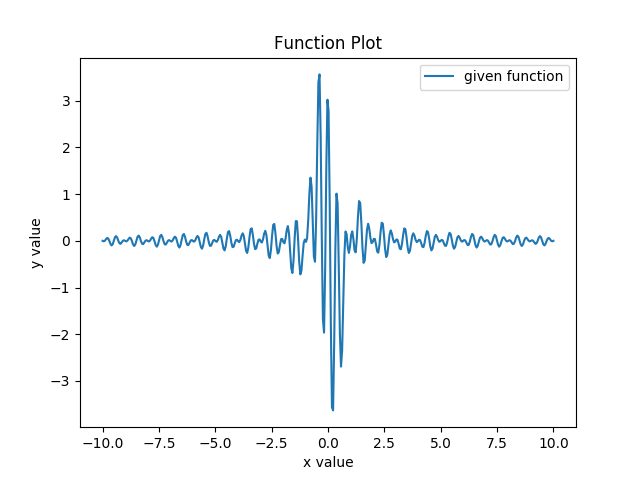
\includegraphics[width=0.75\textwidth]{functionplot400.png}
	\caption{Function Plot}
\end{figure}\\
The analytic derivative was calculated, and is also plotted below
\begin{figure}[h]
	\centering
	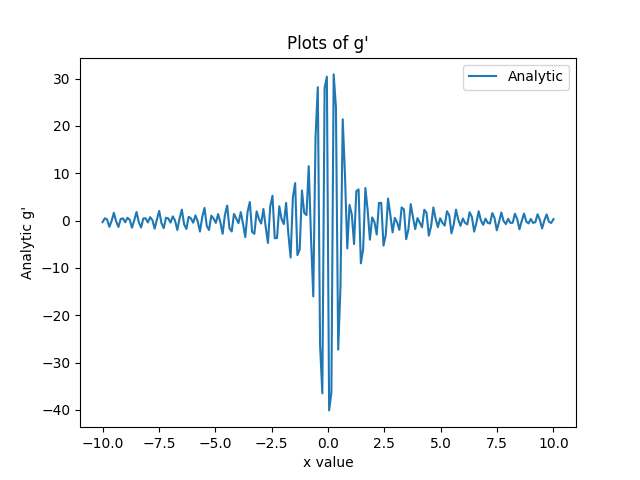
\includegraphics[width=0.45\textwidth]{gpranalytic.png}
	\caption{Analytic derivative}
\end{figure}\\\\
The forward, backward and central difference methods were employed for the function $g(x)$ to compute the derivative. The overlapping plots of the three methods, along with the analytic solution is presented below. 
\begin{figure}[h]
	\centering
	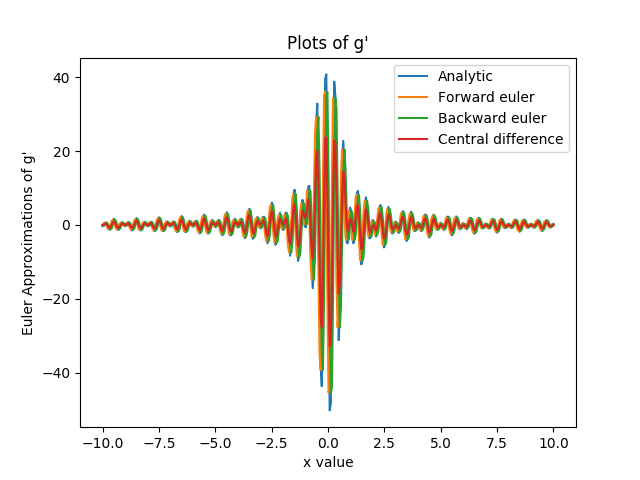
\includegraphics[width=0.60\textwidth]{gprimeeulerplot400.png}
	\caption{Euler Approximations}
\end{figure}\\\\\\
Plotted below are the average and percent error with respect to $x$ 
\begin{figure}[h]
	\centering
	\begin{subfigure}[h]{0.40\textwidth}
		\centering
		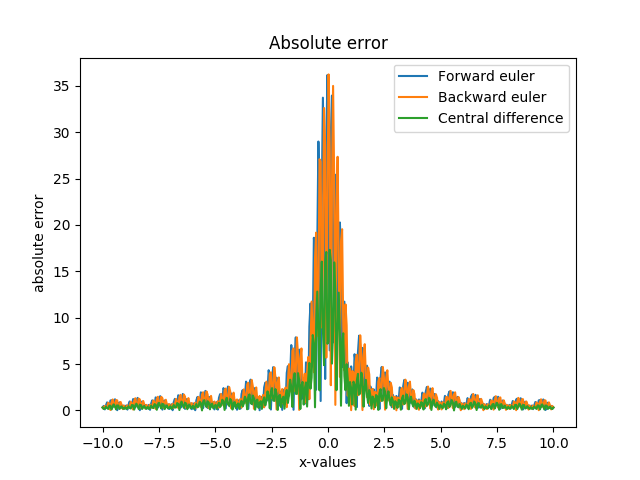
\includegraphics[width=\textwidth]{gprimeabserror400.png}
		\caption{Absolute Error }
	\end{subfigure}
	\begin{subfigure}[h]{0.40\textwidth}
		\centering
		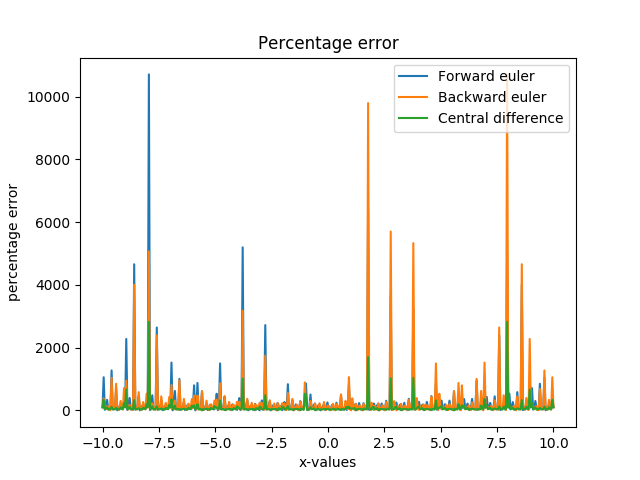
\includegraphics[width=\textwidth]{gprimepercenterror400.png}
		\caption{Percent error}
	\end{subfigure}
	\caption{Error Plots}
\end{figure}

Notice that the number of spikes in percent error has gone up significantly. This is because, with a finer grid spacing, we are hitting a lot of $x$ values where $g'(x)$ is very close to zero. However, the most important thing to notice is that the percentage error has significantly gone down. This is simply because as we get closer to points where $g'$ is zero, we have closer and closer approximations, and thus the approximated solution is much closer to the analytic solution, and thus dividing by the analytic solution does not create as big an impact as it did with coarser grid spacing. Notice also that the magnitude of the absolute error has gone down significantly as well. This is justified by the very same reason. Needless to say, the central difference method outperforms the other two methods in this setting as well. \\\\
The average errors (for Forward Euler, backward Euler and central-difference respectively) reported are as follows 
\begin{figure}[h]
	\centering
	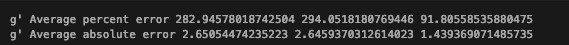
\includegraphics[width=0.60\textwidth]{errorgpr400.png}
	\caption{Average errors}
\end{figure}\\\\
Notice that the average percentage error has gone down by a significant amout. This is once again apparent from the reasons we discussed above. It is however interesting to see a slight increase in the absolute errors pertaining to forward and backward euler methods. This could be because of various reasons, one in particular being that we sample x-values where a lot more of them have $g'(x)$ very close to zero, with euler methods producing non-zero solutions. 
\\\\
The same steps as above was done for computing the second derivative of the function. The forward, backward and central difference methods were employed for the function $g'(x)$ to compute the derivative. The overlapping plots of the three methods, along with the analytic solution is presented below. 
\begin{figure}[h]
	\centering
	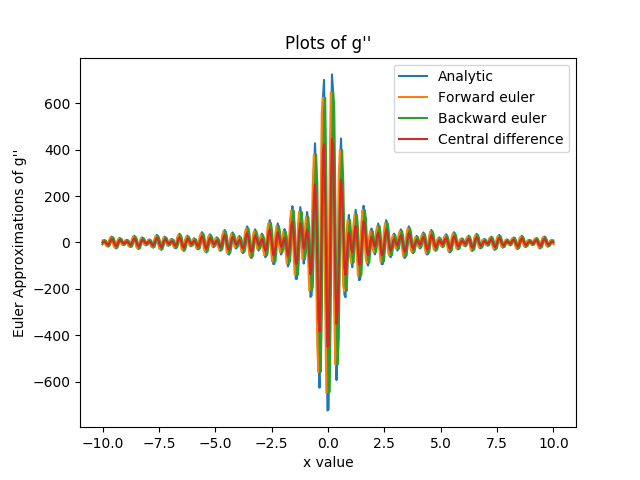
\includegraphics[width=0.60\textwidth]{gdprimeeulerplot400.png}
	\caption{Euler Approximations}
\end{figure}\\\\
Plotted below are the average and percent error with respect to $x$ 
\begin{figure}[h]
	\centering
	\begin{subfigure}[h]{0.40\textwidth}
		\centering
		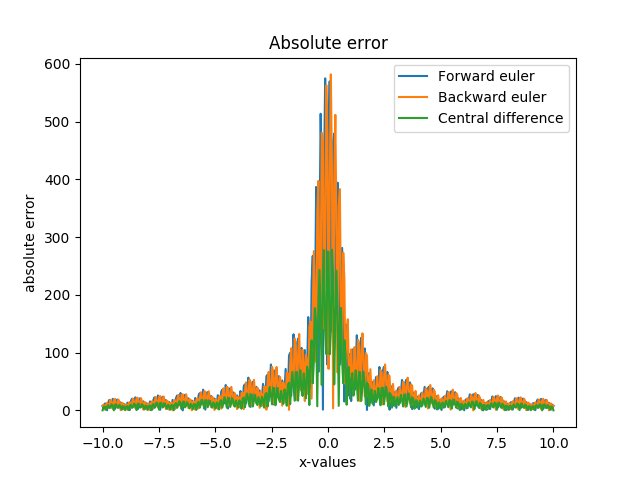
\includegraphics[width=\textwidth]{gdprimeabserror400.png}
		\caption{Absolute Error }
	\end{subfigure}
	\begin{subfigure}[h]{0.40\textwidth}
		\centering
		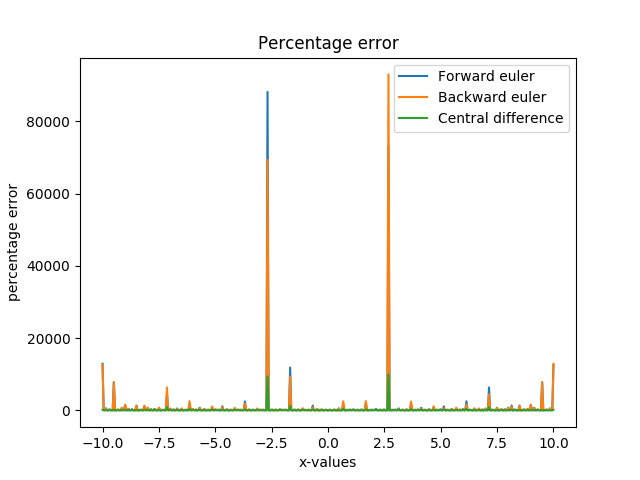
\includegraphics[width=\textwidth]{gdprimepercenterror400.png}
		\caption{Percent error}
	\end{subfigure}
	\caption{Error Plots}
\end{figure}\\\\\\\\\\\\\\\\
It is clear that, once again the central difference method performs much better than both foward and backward euler methods, for the same reasons as before \\\\
We notice more spikes in the percentage errors here again, because like we noticed $g'(x)$ varies very rapidly, and thus will have a lot of points where it plummets to zero. In addition, the additional grid spacing are not helping because we sample more points that are very close to zero. Forward and backward euler methods do not particularly work well in this scenario, and thus resulting in huge spikes with a comparably lesser magnitude than the ones in the case of $g'$. The lesser magnitude can once again be attributed to there being a more refined data in this scenario. \\\\
The average errors (for Forward Euler, backward Euler and central-difference respectively) reported are as follows 
\begin{figure}[h]
	\centering
	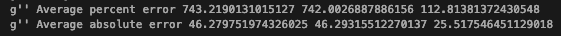
\includegraphics[width=0.60\textwidth]{errorgdpr400.png}
	\caption{Average errors}
\end{figure}\\\\
We notice that the average percent error has significantly gone up from the case of $g''$ when $n=200$, and this is because like we noted - $g''$ behaves very violently, and with more grid points, we have a lot more data points were the function becomes very close to zero which is undesirable for forward and backward euler. The absolute errors have also gone up because of the additional scale factors that we obtain upon taking the second derivative - and so the absolute errors naturally scale up. The huge spikes that we notice in the percentage error is because of our sampled $x$ value being very close to zero (this time in the order of $10^{-3}$), whereas in the previous case, we simply jumped over this data point, and picked the two neighbors of it, thus avoiding this problem (by accident). However, negating the huge spikes (throwing out the anamolies from the data) in both cases, we have the average percent error in $n=400$ case being lower than in the case of $n=200$ as expected. \\\\

\textbf{(2 a)}
In order to compute the fourier transform of $g$, the number of $x$ values being considered had to be changed. It was changed to $1024 = 2^{10}$. This sampling will allow for an efficient fft. The FFT library provided by numpy was used for this purpose. The negative frequencies are filtered out in the process as they are not of physical significance. The unscaled FT plot (in both time and frequency domain) is reproduced below. 
\begin{figure}[h]
	\centering
	\begin{subfigure}[h]{0.40\textwidth}
		\centering
		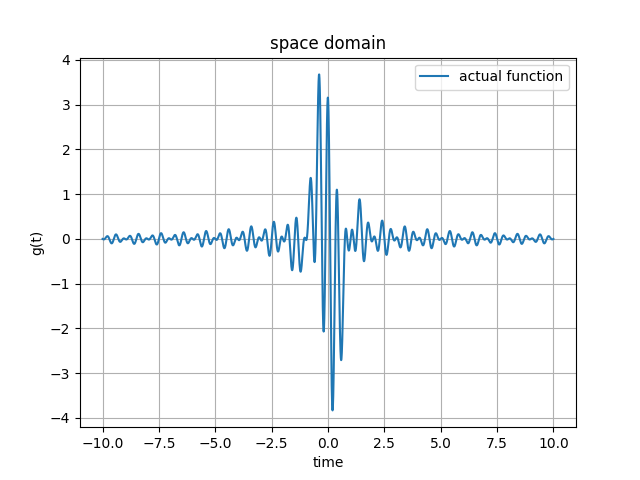
\includegraphics[width=\textwidth]{space_domain_actualfunc1024.png}
		\caption{Space Domain }
	\end{subfigure}
	\begin{subfigure}[h]{0.40\textwidth}
		\centering
		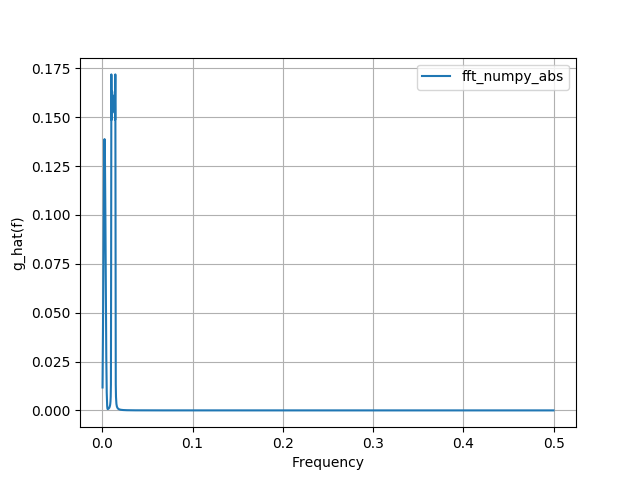
\includegraphics[width=\textwidth]{freq_domain_numpy.png}
		\caption{Frequency Domain}
	\end{subfigure}
	\caption{FFT Plots}
\end{figure}
Upon rescaling we should be able to obtain the correct frequencies from the FFT plot. Since the original frequencies are hard to compute for the given function, it becomes hard to justify the frequencies in the FFT plot. \\\\ For a proof of concept, consider the simple function $4\sin(10\pi x) + 3\cos(20\pi x)$ and a shift of it $4\sin(10\pi (x-0.25)) + 3\cos(20\pi (x-0.25))$. The two functions are plotted below along with their FFT. The sampled number of data points were 1024.
\begin{figure}[h]
	\centering
	\begin{subfigure}[h]{0.40\textwidth}
		\centering
		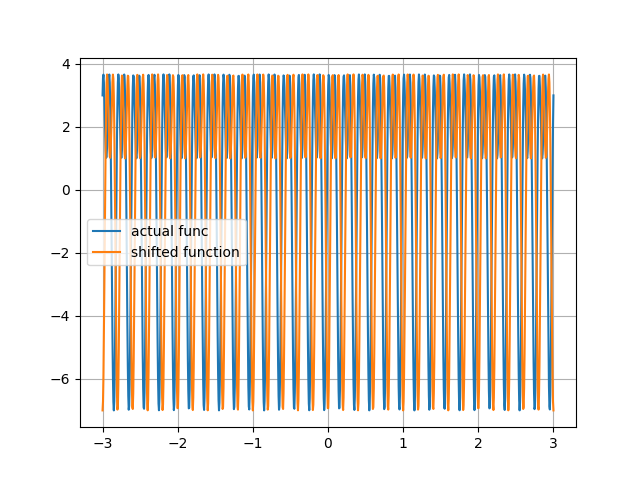
\includegraphics[width=\textwidth]{POC_space_domain.png}
		\caption{Space Domain }
	\end{subfigure}
	\begin{subfigure}[h]{0.40\textwidth}
		\centering
		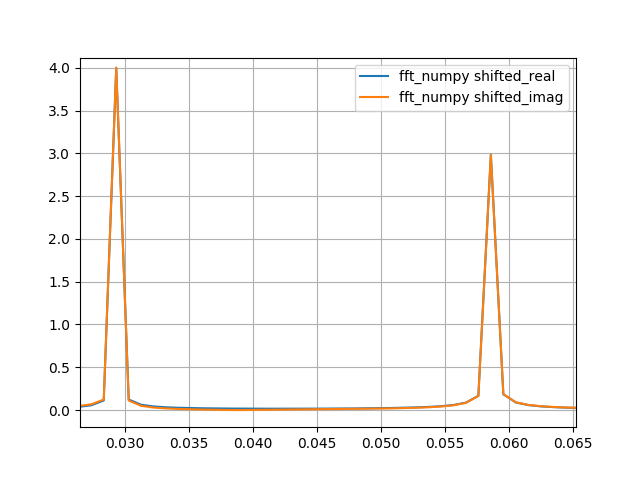
\includegraphics[width=\textwidth]{POC_freq.png}
		\caption{Frequency Domain}
	\end{subfigure}
	\caption{Proof of concept}
\end{figure}
Notice that in the FFT plot here, the peaks occur at $\simeq 0.0299$ and $\simeq 0.0598$, and we have $\frac{10\pi}{1024} = 0.03067$ and $\frac{20\pi}{1024} = 0.06135$. The little error we see can be attributed to numerical errors that are transferred while travelling to the frequency domain. This proves that rescaling does return the desired frequencies. \\
\textbf{(2 b)} The first derivative of the function was calculated using spectral methods, and the output is plotted along with the analytic derivative. The plot is reproduced below. 
\begin{figure}[h]
	\centering
	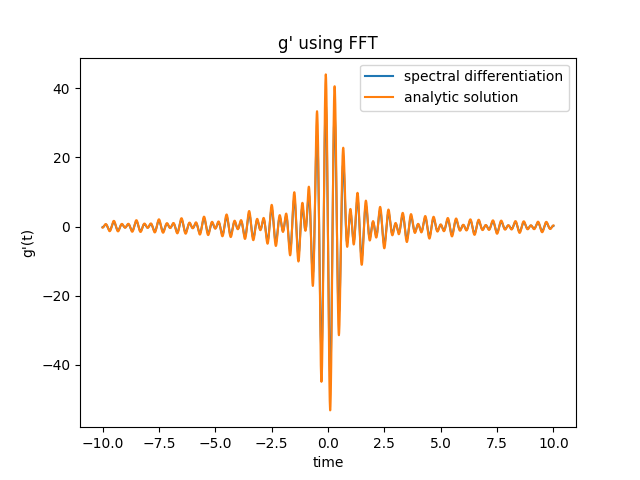
\includegraphics[width=0.60\textwidth]{fftanalyticcomparison.png}
	\caption{Spectral method and analytic derivative}
 \end{figure}\\\\
It is apparent from the plot that the error was very close to zero (that is to say, the spectral method produced the exact analytic derivative) with very small numerical errors. \\\\
\textbf{(2 c)} The plot obtained through the spectral method was then plotted alongside the Euler approximations obtained in 1 c. The plot is reproduced below. \\ 
\begin{figure}[h]
	\centering
	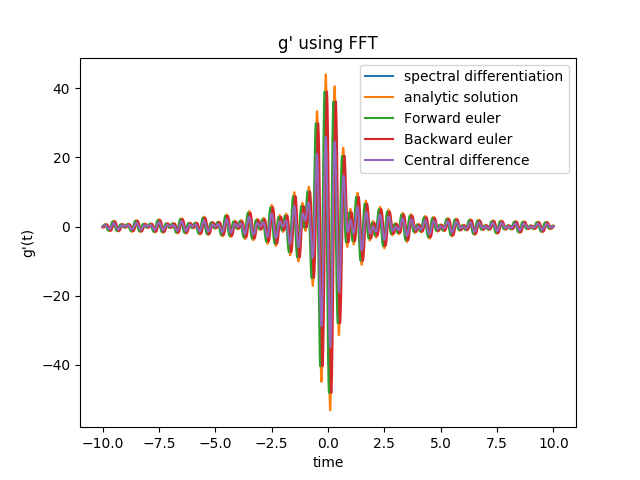
\includegraphics[width=0.40\textwidth]{eulerfftcomparison.png}
	\caption{Spectral method vs Euler approximations}
\end{figure}\\\\
Upon computing the error, the maximum absolute error that was reported was $33.30, 32.56$ and $9.11$ for Forward Euler, Backward Euler and Central difference respectively. Once again, we see the central difference outperforming the forward and backward euler. \\\\
\textbf{(3 a)} Given $f(x) = ae^{bx}$. Upon fitting the function with an exponential fit, we obtain the values of $a$ and $b$ as $a = 3.64404617$ and $b = 0.54550424$. The fitted function along with the data is plotted below. 
\begin{figure}[h]
	\centering
	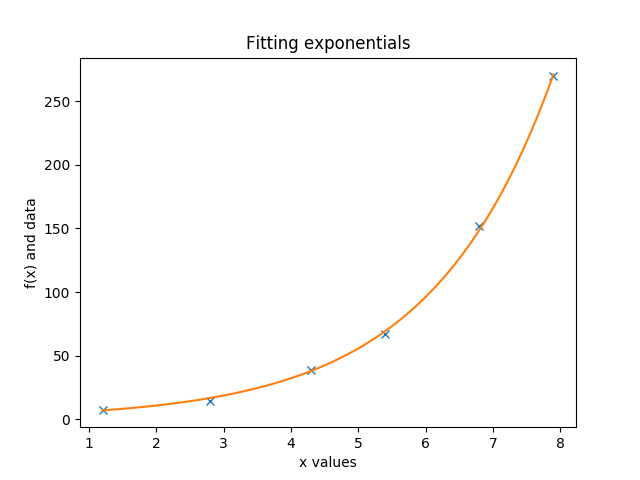
\includegraphics[width=0.50\textwidth]{exp_fitting.png}
	\caption{Exponential fitting}
\end{figure}\\\\
\textbf{(3 b)} The data was then interpolated, using a cubic spline interpolation to the given points and the values returned were as follows: $f(1.3) = 6.9971847, f(2.9) = 15.3595104, f(4.4) = 40.8406263, f(5.5) = 70.876742$ and $f(6.9) = 160.54950$ \\\\
A cubic interpolating spline $s$ is a cubic polynomial that has the property that $s(x_m) = f(x_m)$, with the additional condition that $s''(x_0) = s''(x_m) =0$. This helps in smoothing of the spline, thereby getting a better estimate than regular polynomial interpolation which might have differentiability issues at the data points. 
We construct the spline by solving the following system\\\\
$s_i = a_i(x-x_i) + b_i(x-x_i)^2 + c_i(x-x_i) + d_i$. \\ By fixing the $4m$ coefficients ($a_i, b_i, c_i, d_i$ as $i: 0 \rightarrow m-1$), we fix the spline. This is a linear system solved in the following fashion with $4m$ conditions being \\\\
$s''(x_0) = s''(x_m) = 0$\\
$s_i(x_i) = y_i$\\
$s_{m-1} = y_m$\\
$s_i(x_{i+1}) = s_{i+1}(x_{i+1})$\\
$s'_i(x_{i+1}) = s'_{i+1}(x_{i+1})$\\
$s''_i(x_{i+1}) = s''_{i+1}{x_{i+1}}$\\\\
I chose the cubic spline interpolation, because it is the highest order spline interpolation provided by the interp1d function in numpy, and is very easy to impliment. The given function being non-polynomial, I realized that the highest order polynomial approximation available will minimize the errors. Plotted below is the interpolated spline.
 \begin{figure}[h]
 	\centering
 	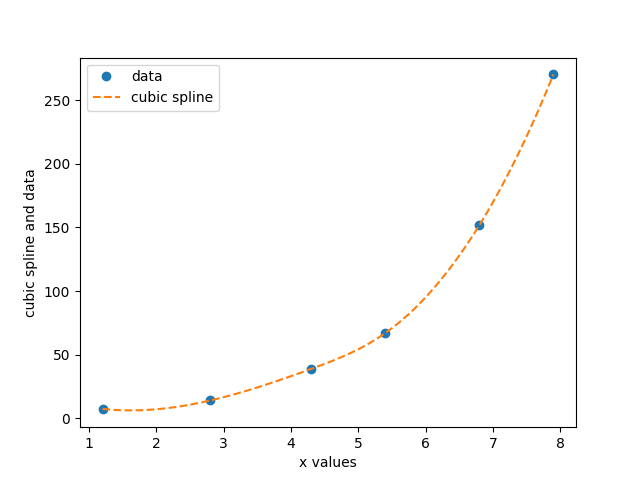
\includegraphics[width=0.50\textwidth]{cubic_spline.png}
 	\caption{Cubic Spline interpolation}
 \end{figure}\\\\ 
\textbf{(1 c)} The average absolute error between the fitted function and the interpolating function was reported to be $1.8387$ and the average percentage error between the two was reported to be $5.1770$.\\\\
Interpolation is a method of constructing new data points within the range of a set of known data points, whereas fitting data refers to the process of finding a curve that best represents the trend of the data (or in other words, best "fits" the data). In other words, given some data - interpolation is the process of constructing a curve through the data points with the implicit assumption that the data points are accurate. Curve fitting, on the other hand applied to data that contains noise, will return a smooth curve that approximates the data and its trend.
\newpage 
\begin{center}
APPENDIX 1 
\end{center}
\noindent \textbf{4(a)}\lstinputlisting[language=Python]{compphysmidterm.py}


\newpage  
\noindent \textbf{4(b)}\lstinputlisting[language=Python]{compphysmidterm3.py}

\end{document}